\documentclass{beamer}
\usetheme{Rochester}
\addtobeamertemplate{navigation symbols}{}{ \hspace{1em}    \usebeamerfont{footline}%
	\insertframenumber / \inserttotalframenumber }
\begin{document}
	\title{Introduction to Probabilistic Record Linkage}
	%\subtitle{Using Beamer}
	\author{Brian Kundinger, Jerome Reiter, Rebecca Steorts}
	\institute{Duke University}
	\date{\today}
	
%	\AtBeginSection[]{
%		\begin{frame}
%			\vfill
%			\centering
%			\begin{beamercolorbox}[sep=8pt,center,shadow=true,rounded=true]{title}
%				\usebeamerfont{title}\insertsectionhead\par%
%			\end{beamercolorbox}
%			\vfill
%		\end{frame}
%	}

\AtBeginSection[]
{
	\begin{frame}
		\frametitle{Table of Contents}
		\tableofcontents[currentsection]
	\end{frame}
}
	
	\begin{frame}
		\titlepage
	\end{frame}

%	\begin{frame}
%	\frametitle{Outline}
%	\tableofcontents
%	\end{frame}

\section{Introduction to Record Linkage}

	\begin{frame}{What is Record Linkage?}
	\begin{itemize}
		\item Record linkage is the task of identifying duplicate records over noisy datasets.
		
		\item Easy with unique identifiers, difficult when faced with errors
		
		\item \textbf{Bipartite matching} is the specific goal of matching one record in one dataset to most one match in another dataset
	\end{itemize}
	\end{frame}


%\begin{frame}{Record Linkage in Practice}
%	\begin{columns}
%		\begin{column}{0.48\textwidth}
%			\includegraphics<1->[width = \textwidth, height = .9\textwidth ]{ted_article2.png}
%			
%		\end{column}
%		\begin{column}{0.48\textwidth}
%			\includegraphics<2->[width = \textwidth, height = .9\textwidth ]{dnc_header.png}
%		\end{column}
%	\end{columns}
%\end{frame}

\begin{frame}{Record Linkage in Practice}
	\centering
	\includegraphics<1->[width = .8\textwidth, height = .6\textwidth ]{graphics/syria_article_big.png}
\end{frame}

\begin{frame}{Linkage for Downstream Analysis}
	\includegraphics<1>[width = \textwidth, height = .7\textwidth ]{graphics/Slide1.png}
	\includegraphics<2>[width = \textwidth, height = .7\textwidth ]{graphics/Slide2.png}
\end{frame}

\begin{frame}{Linkage through Comparison Vectors}
	\includegraphics<1>[width = \textwidth, height = .6\textwidth ]{graphics/Slide3.png}
	\includegraphics<2>[width = \textwidth, height = .6\textwidth ]{graphics/Slide4.png}
	\includegraphics<3>[width = \textwidth, height = .6\textwidth ]{graphics/Slide5.png}
\end{frame}

\begin{frame}{Linkage through Comparison Vectors}
	Represent linkage structure through vector $\mathbf{Z} = \{Z_1, \ldots, Z_{n_B}\}$, where
\begin{center}
	$Z_j = \begin{cases} 
		i,  & \text{if records } i\in A \text{ and } j\in B \text{ match}; \\
		n_A + 1,  & \text{if record } j\in B \text{ has no match in } A; \\
	\end{cases}$
\end{center}
\end{frame}

\begin{frame}{Linkage through Comparison Vectors}
	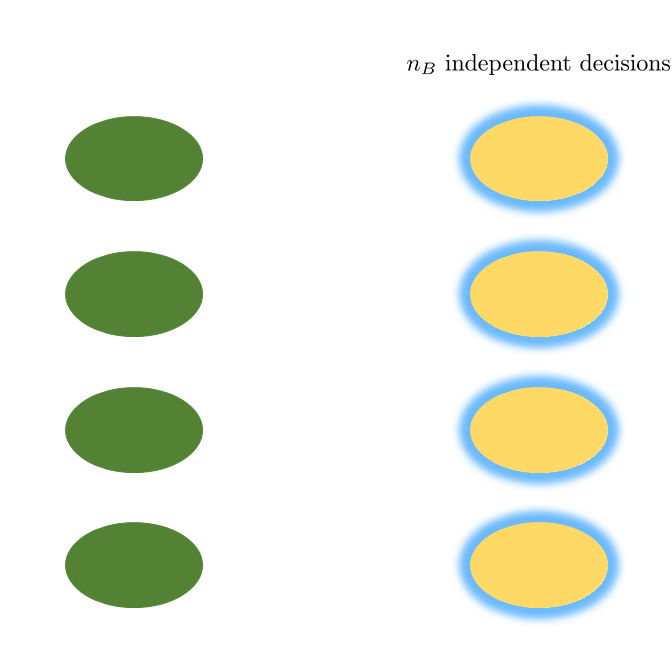
\includegraphics[width = \textwidth, height = .6\textwidth ]{graphics/Slide6.png}
\end{frame}

\begin{frame}{Fellegi and Sunter (1969)}
	\begin{columns}
		\begin{column}{0.6\textwidth}
			\includegraphics<1>[width = \textwidth, height = 1.2\textwidth ]{graphics_square/Slide1.png}
			\includegraphics<2->[width = \textwidth, height = 1.2\textwidth ]{graphics_square/Slide2.png}
		\end{column}
		\begin{column}{0.38\textwidth}
			\begin{itemize}
				\item<3-> scalable to large datasets (\texttt{fastlink}, Enamorado et al 2019)
				\item<4-> not bipartite, requires post-processing
				\pause 
				\item<5-> overmatches, leading to inaccurate parameter estimation
			\end{itemize}

		\end{column}
	\end{columns}
\end{frame}

\begin{frame}{Fellegi and Sunter (1969)}
	\begin{itemize}
		\item The Fellegi and Sunter model is essentially a \emph{mixture model}
		\item We posit that comparison vectors come from two different distributions, one for matching, and another for nonmatching record pairs
		\item The model learns the parameters for each distribution and independently classifies each record pair as matching or nonmatching.
	\end{itemize}
\end{frame}

\begin{frame}{Sadinle (2017)}
	\begin{columns}
		\begin{column}{0.6\textwidth}
			\includegraphics<1>[width = \textwidth, height = 1.2\textwidth ]{graphics_square/Slide1.png}
			\includegraphics<2>[width = \textwidth, height = 1.2\textwidth ]{graphics_square/Slide3.png}
			\includegraphics<3>[width = \textwidth, height = 1.2\textwidth ]{graphics_square/Slide4.png}
			\includegraphics<4->[width = \textwidth, height = 1.2\textwidth ]{graphics_square/Slide5.png}
		\end{column}
		\begin{column}{0.38\textwidth}
			\begin{itemize}
				\item<1-> Beta Record Linkage (\texttt{BRL})
				\pause
				\item<5-> strictly enforces one-to-one matching, no post-processing
				\pause
				\item<6-> high accuracy for linkage and other parameters
				\pause 
				\item<7-> inherently serial, not scalable to large linkage tasks
			\end{itemize}
			
		\end{column}
	\end{columns}
\end{frame}

\begin{frame}{Our Contribution - Fast Beta Linkage}
	\begin{columns}
		\begin{column}{0.6\textwidth}
			\includegraphics<1>[width = \textwidth, height = 1.2\textwidth ]{graphics_square/Slide1.png}
			\includegraphics<2-4>[width = \textwidth, height = 1.2\textwidth ]{graphics_square/Slide6.png}
			\includegraphics<5>[width = \textwidth, height = 1.2\textwidth ]{graphics_square/Slide7.png}
			\includegraphics<6>[width = \textwidth, height = 1.2\textwidth ]{graphics_square/Slide8.png}
		\end{column}
		\begin{column}{0.38\textwidth}
			\begin{itemize}
				\item<3-> relaxation proposed by Heck Wortman (2019)
				\item<4-> minimal loss of accuracy, large computational gains
				\item<5-> allows for "one to many" matchings
				\item<6-> simple postprocessing to obtain bipartite matching
			\end{itemize}
			
		\end{column}
	\end{columns}
\end{frame}

\begin{frame}{Model Parameters}
	\begin{itemize}
		\item Both models utilize $\mathbf{m}$ and $\mathbf{u}$ parameters to model the data.
		\item Define $m_{f\ell} = P(\gamma_{ij}^f = \ell | \text{Records Match})$ and $u_{f\ell} = P(\gamma_{ij}^f = \ell | \text{Records Do Not Match})$
		\item We can think of $\mathbf{m}$ as reliability parameters, that show how likely it is for a feature to remain unchanged across files
		\item We can think of $\mathbf{u}$ as discernment parameters, that show how unique the values of a feature can be
	\end{itemize}
\end{frame}

\begin{frame}{Fellegi Sunter Weights}
	\begin{itemize}
		\item We multiply these parameters for all $f$ and the relevant $\ell$ to get $\mathbf{m}_{ij} = P(\gamma_{ij}| \text{Records Match})$ and $\mathbf{u}_{ij} = P(\gamma_{ij}| \text{Records Do Not Match})$
		\item These probabilities form the likelihood ratio 
		$$w_{ij} = \frac{P(\gamma_{ij}| \text{Records Match})}{P(\gamma_{ij}| \text{Records Do Not Match})}$$
		\item This ratio is large when $\mathbf{m}_{ij}$ is large and $\mathbf{u}_{ij}$ is small
	\end{itemize}
\end{frame}

\section{Practical Considerations}

\begin{frame}{Constructing Comparison Vectors}
	\begin{itemize}
		\item We measure the distance between two fields using whatever metric we like, and then threshold this distance into discrete values
		\item We can use binary agreement, or use multiple agreement levels to capture partial agreement
		\item Existing packages perform binary agreement, numerical distance, and string distance
	\end{itemize}
\end{frame}

\begin{frame}{String Distance}
	\begin{itemize}
		\item Many packages compare strings through the normalized Levenstein distance. This is the minimum number of edits required to transform one string to the other, divided by the length of the larger string.
		\item Additional metrics could be language specific Soundex codes
		\item Care should be taken when transforming metric into discreet agreement level. For example, should a Soundex match be regarded as a full match or a partial match?
		\item Code from existing packages can be edited to accomodate additional string distances
	\end{itemize}
\end{frame}

\begin{frame}{Conditionally Independent Features}
	\begin{itemize}
		\item The record linkage model assumes that agreement levels are \emph{conditionally independent}, given the matching status of the records. This is satisfied for most fields
		\item For example, knowing that two records agree on birth month does not tell you anything about whether they agree on birth year. These fields are independent
		\item In contrast, if two records disagree on department, we know they probably disagree on city. These fields are not independent
		\item Using dependent features is essentially using the same information multiple times, and can harm results
	\end{itemize}
\end{frame}

\begin{frame}{Conditionally Independent Features}
	\begin{itemize}
		\item One solution to dependent features is to create a more nuanced comparison incorporating multiple features
		\item For example, you can define full agreement for "location" to be matching on city AND department, partial agreement to be matching on only department, and no agreement not be matching on neither.
		\item Current packages do not execute this type of comparison, but this can be done with some work
		\item Depending on the type of dependent fields, I may recommend keeping both or just omitting one. 
	\end{itemize}
\end{frame}

\begin{frame}{Conditionally Independent Features}
	\begin{itemize}
		\item One solution to dependent features is to create a more nuanced comparison incorporating multiple features
		\item For example, you can define full agreement for "location" to be matching on city AND department, partial agreement to be matching on only department, and no agreement not be matching on neither.
		\item Current packages do not execute this type of comparison, but this can be done with some work
		\item Depending on the type of dependent fields, I may recommend keeping both or just omitting one. 
	\end{itemize}
\end{frame}

\begin{frame}{Random Sampling and Generalization}
	\begin{itemize}
		\item To avoid calculating $n_A n_B$ comparison vectors, we can use \emph{blocking}
		\item We only create comparison vectors when records agree on a particular field
		\item It may be tempting to block on a unique identifier, but this can create blocks that are too small for record linkage to run effectively
	\end{itemize}
\end{frame}

\begin{frame}{Thoughts for DANE}
	\begin{itemize}
		\item With \texttt{fastLink}, you may be able to do the entire linkage task (60,000 $\times$ 1,000,000) records at one time. If not blocking by gender or by department should make it feasible
		\item You should not need to use the generalization technique
		\item \texttt{fastLink} currently does not do Soundex comparisons, but using allowing for partial agreement on strings should be sufficient. \texttt{fastLink} code can be modified to incorporate Soundex comparison, but may take some work
	\end{itemize}
\end{frame}

\section{Evaluation}

\begin{frame}{Performance Metrics with Known Labels}
	\begin{itemize}
		\item When true matching status is known, we use two primary metrics:
		\begin{itemize}
		\item $\text{Recall} = \frac{\text{True Matches Declared}}{\text{Total True Matches}}$
		\item $\text{Precision} = \frac{\text{Matches Declared}}{\text{Total Matches Declared}}$
		\end{itemize}
		\item To balance these two metrics, we sometimes also consider:
		\begin{itemize}
		\item  $\text{F-Measure} = \frac{\text{Recall} \times \text{Precision}}{\text{Recall} + \text{Precision}}$
		\end{itemize}
	\end{itemize}
\end{frame}

\begin{frame}{Performance Metrics without Known Labels}
	\begin{itemize}
		\item Without known labels, evaluating model performance is more difficult, but there are general checks you can make
		\begin{itemize}
			\item The histogram of match probabilities should be clearly separated, with most record pairs having probabilities near 0 or near 1, and minimal number of pairs in between
			\item  Fellegi Sunter weights for impactful matching variables should be high. Weights for partial agreement should be lower than those for full agreement
			\item Visually inspect a subset of matches and nonmatches. In particular, examine matches near the decision threshold.
		\end{itemize}
	\item These approaches are demonstrated in the accompanying Rmarkdown file
	\end{itemize}
\end{frame}

\section{Software}
\begin{frame}{Software}
	\begin{itemize}
		\item \texttt{fastLink} can be found on \href{https://github.com/kosukeimai/fastLink}{GitHub}
		\item \texttt{BRL} can also be found on \href{https://github.com/cran/BRL}{GitHub}
		\item \texttt{fabl} is not yet publicly available
		\item Due to the scale of DANE's record linkage task, I recommend you to use \texttt{fastLink}
	\end{itemize}
\end{frame}

\section{References}
\begin{frame}{References}
	\begin{itemize}
		\item Fellegi I. and Sunter A., A theory for record linkage, J. Am. Stat. Assoc. 64 (1969), pp. 1183–1210
		\item Enamorado T., Fifield B. and Imai K., Using a probabilistic model to assist merging of large-scale administrative records, Am. Political Sci. Rev. 113 (2019), pp. 353–371
		\item Sadinle M., Bayesian estimation of bipartite matchings for record linkage, J. Am. Stat. Assoc. 112 (2017), pp. 600–612
	\end{itemize}
\end{frame}

\end{document}